\documentclass[tikz,border=10pt]{standalone}
% Trapezoid ABCD with AD parallel to BC (horizontal).
% Scale s = 0.013333 cm/px (longest side of ink bbox = 8 cm), y axis flipped.
% Coordinates use bbox centre (375, 237.5) as origin.
\begin{document}
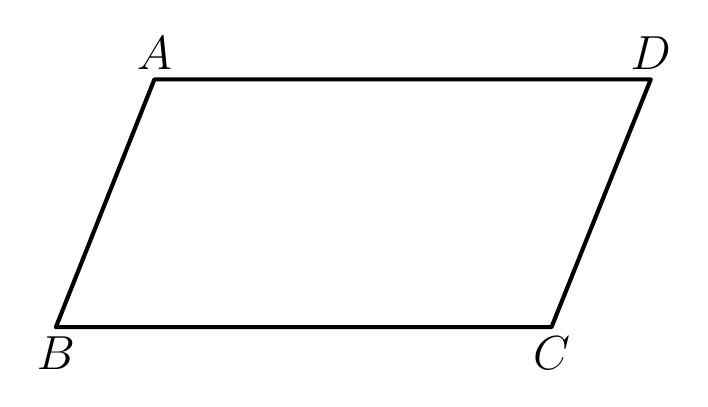
\begin{tikzpicture}[line join=round]
  % Vertices (from pixel coordinates)
  \coordinate (A) at (-2.528,  1.580);
  \coordinate (D) at ( 3.776,  1.580);
  \coordinate (B) at (-3.779, -1.567);
  \coordinate (C) at ( 2.515, -1.567);

  % Solid trapezoid outline: AB, BC, CD, DA (no fill)
  \draw[solid, line width=1.5pt] (A) -- (B) -- (C) -- (D) -- cycle;

  % Vertex labels: A and D above, B and C below
  \node[above, font=\fontsize{17}{20.4}\selectfont] at (A) {$A$};
  \node[above, font=\fontsize{17}{20.4}\selectfont] at (D) {$D$};
  \node[below, font=\fontsize{17}{20.4}\selectfont] at (B) {$B$};
  \node[below, font=\fontsize{17}{20.4}\selectfont] at (C) {$C$};
\end{tikzpicture}
\end{document}